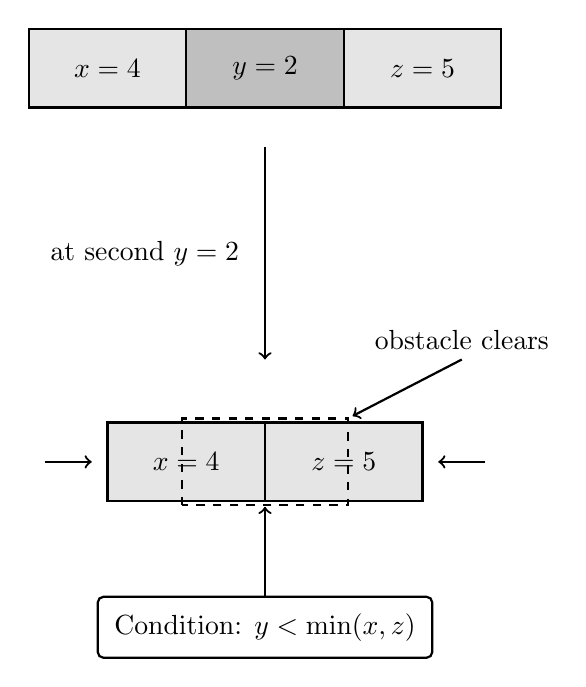
\begin{tikzpicture}

% Top state
\gid{blue-left-block}{
  \draw[thick, fill=black!10] (-3, 3) rectangle (-1, 4);
}
\gid{blue-right-block}{
  \draw[thick, fill=black!10] (1, 3) rectangle (3, 4);
}
\gid{red-middle-block}{
  \draw[thick, fill=black!25] (-1, 3) rectangle (1, 4);
}
\gid{labels-blue-lifetimes}{
  \node at (-2, 3.5) {$x=4$};
  \node at (2, 3.5) {$z=5$};
}
\gid{label-y}{
  \node at (0, 3.5) {$y=2$};
}

% Arrow down
\gid{arrow-down}{
  \draw[->, thick] (0, 2.5) -- (0, -0.2) node[midway, left=0.2cm] {at second $y=2$};
}

% Lower state
\gid{blue-blocks-meeting}{
  \draw[thick, fill=black!10] (-2, -2) rectangle (0, -1);
  \draw[thick, fill=black!10] (0, -2) rectangle (2, -1);
  \node at (-1, -1.5) {$x=4$};
  \node at (1, -1.5) {$z=5$};
  \draw[->, thick] (-2.8, -1.5) -- (-2.2, -1.5);
  \draw[->, thick] (2.8, -1.5) -- (2.2, -1.5);
}

\gid{red-vanishing}{
  \draw[thick, dashed, draw=black] (-1.05, -2.05) rectangle (1.05, -0.95);
}

\gid{label-obstacle-clears}{
  \draw[->, thick, shorten >=2pt] (2.5, -0.2) -- (1.05, -0.95);
  \node[above] at (2.5, -0.2) {obstacle clears};
}

\gid{condition-annotation}{
  \draw[->, thick, shorten >=2pt] (0, -3.2) -- (0, -2);
  \node[below, draw, thick, fill=white, rounded corners=2pt, inner sep=6pt] at (0, -3.2) {Condition: $y < \min(x, z)$};
}

\end{tikzpicture}